\subsection*{Fejlmeddelelse}
Til at vise fejlmeddelelser er der i sekvensdiagrammerne opstillet en midlertidig grænseflade, hvori teksten ændres alt efter, hvilken fejl, der forekommer. Designklassen ses af \autoref{fig:Designfejl}.

\begin{figure} [H]
\centering
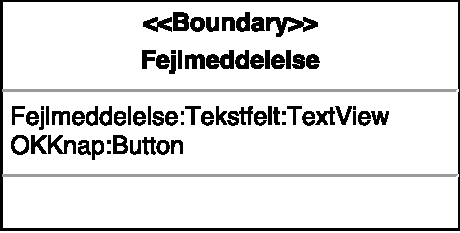
\includegraphics[width=0.2\textwidth]{figures/MVC/MVCfejl}
\caption{Designklasse for fejlmeddelelse.}
\label{fig:Designfejl}
\end{figure}

\noindent
Grænsefladen indeholder en metode makeText. Denne anvendes i log ind, venneliste og redigering af adgangskode til at oplyse brugeren om at indtastede værdier ikke stemmer overens med oplyste værdier i databasen eller ikke eksisterer i databasen. 